\newpage
\section{Laser VCSEL 850\,nm}
Rysunki ~\ref{vcsel_850_rys_1} -- ~\ref{vcsel_850_rys_7} przedstawiają wykresy dla lasera VCSEL 850\,nm. \\
\begin{table}
\begin{center}
\caption{ Wyznaczone wartośc prądu progowego $I_{\mathrm{th}}$ w różnych temperaturach $T$ dla lasera VCSEL 850\,nm.}
\begin{tabular}{ | C{1.5cm}|  C{3.0cm} | C{1.5cm} | C{3.0cm}| C{1.5cm} | C{3.0cm}|}
\hline
$T$ [K] &   $I_{\mathrm{th}}$ [mA]  &  $T$ [K] &   $I_{\mathrm{th}}$ [mA]  &  $T$ [K] &   $I_{\mathrm{th}}$ [mA] 	\\ \hline
283      &   1.70 $\pm$ 0.03  & 288      &   1.67 $\pm$ 0.03   & 293		 &   1.60 $\pm$ 0.03  \\ \hline
298		 &   1.55 $\pm$ 0.04  & 303		 &   1.59 $\pm$ 0.03  & 308		 &   1.63 $\pm$ 0.03  \\ \hline
313		 &   1.65 $\pm$ 0.03  & 318		 &   1.68 $\pm$ 0.04  & 323		 &   1.73 $\pm$ 0.04  \\ \hline
328		 &   1.83 $\pm$ 0.04  & 333		 &   1.89 $\pm$ 0.04  & 338		 &   2.01 $\pm$ 0.04  \\ \hline
343		 &   2.14 $\pm$ 0.04  & 348		 &   2.24 $\pm$ 0.05  & 353		 &   2.38 $\pm$ 0.05  \\ \hline
358		 &   2.57 $\pm$ 0.05  & 363		 &   2.74 $\pm$ 0.07  \\ \cline{1-4}
\end{tabular}
\end{center}
\end{table}
\begin{figure}
\center
  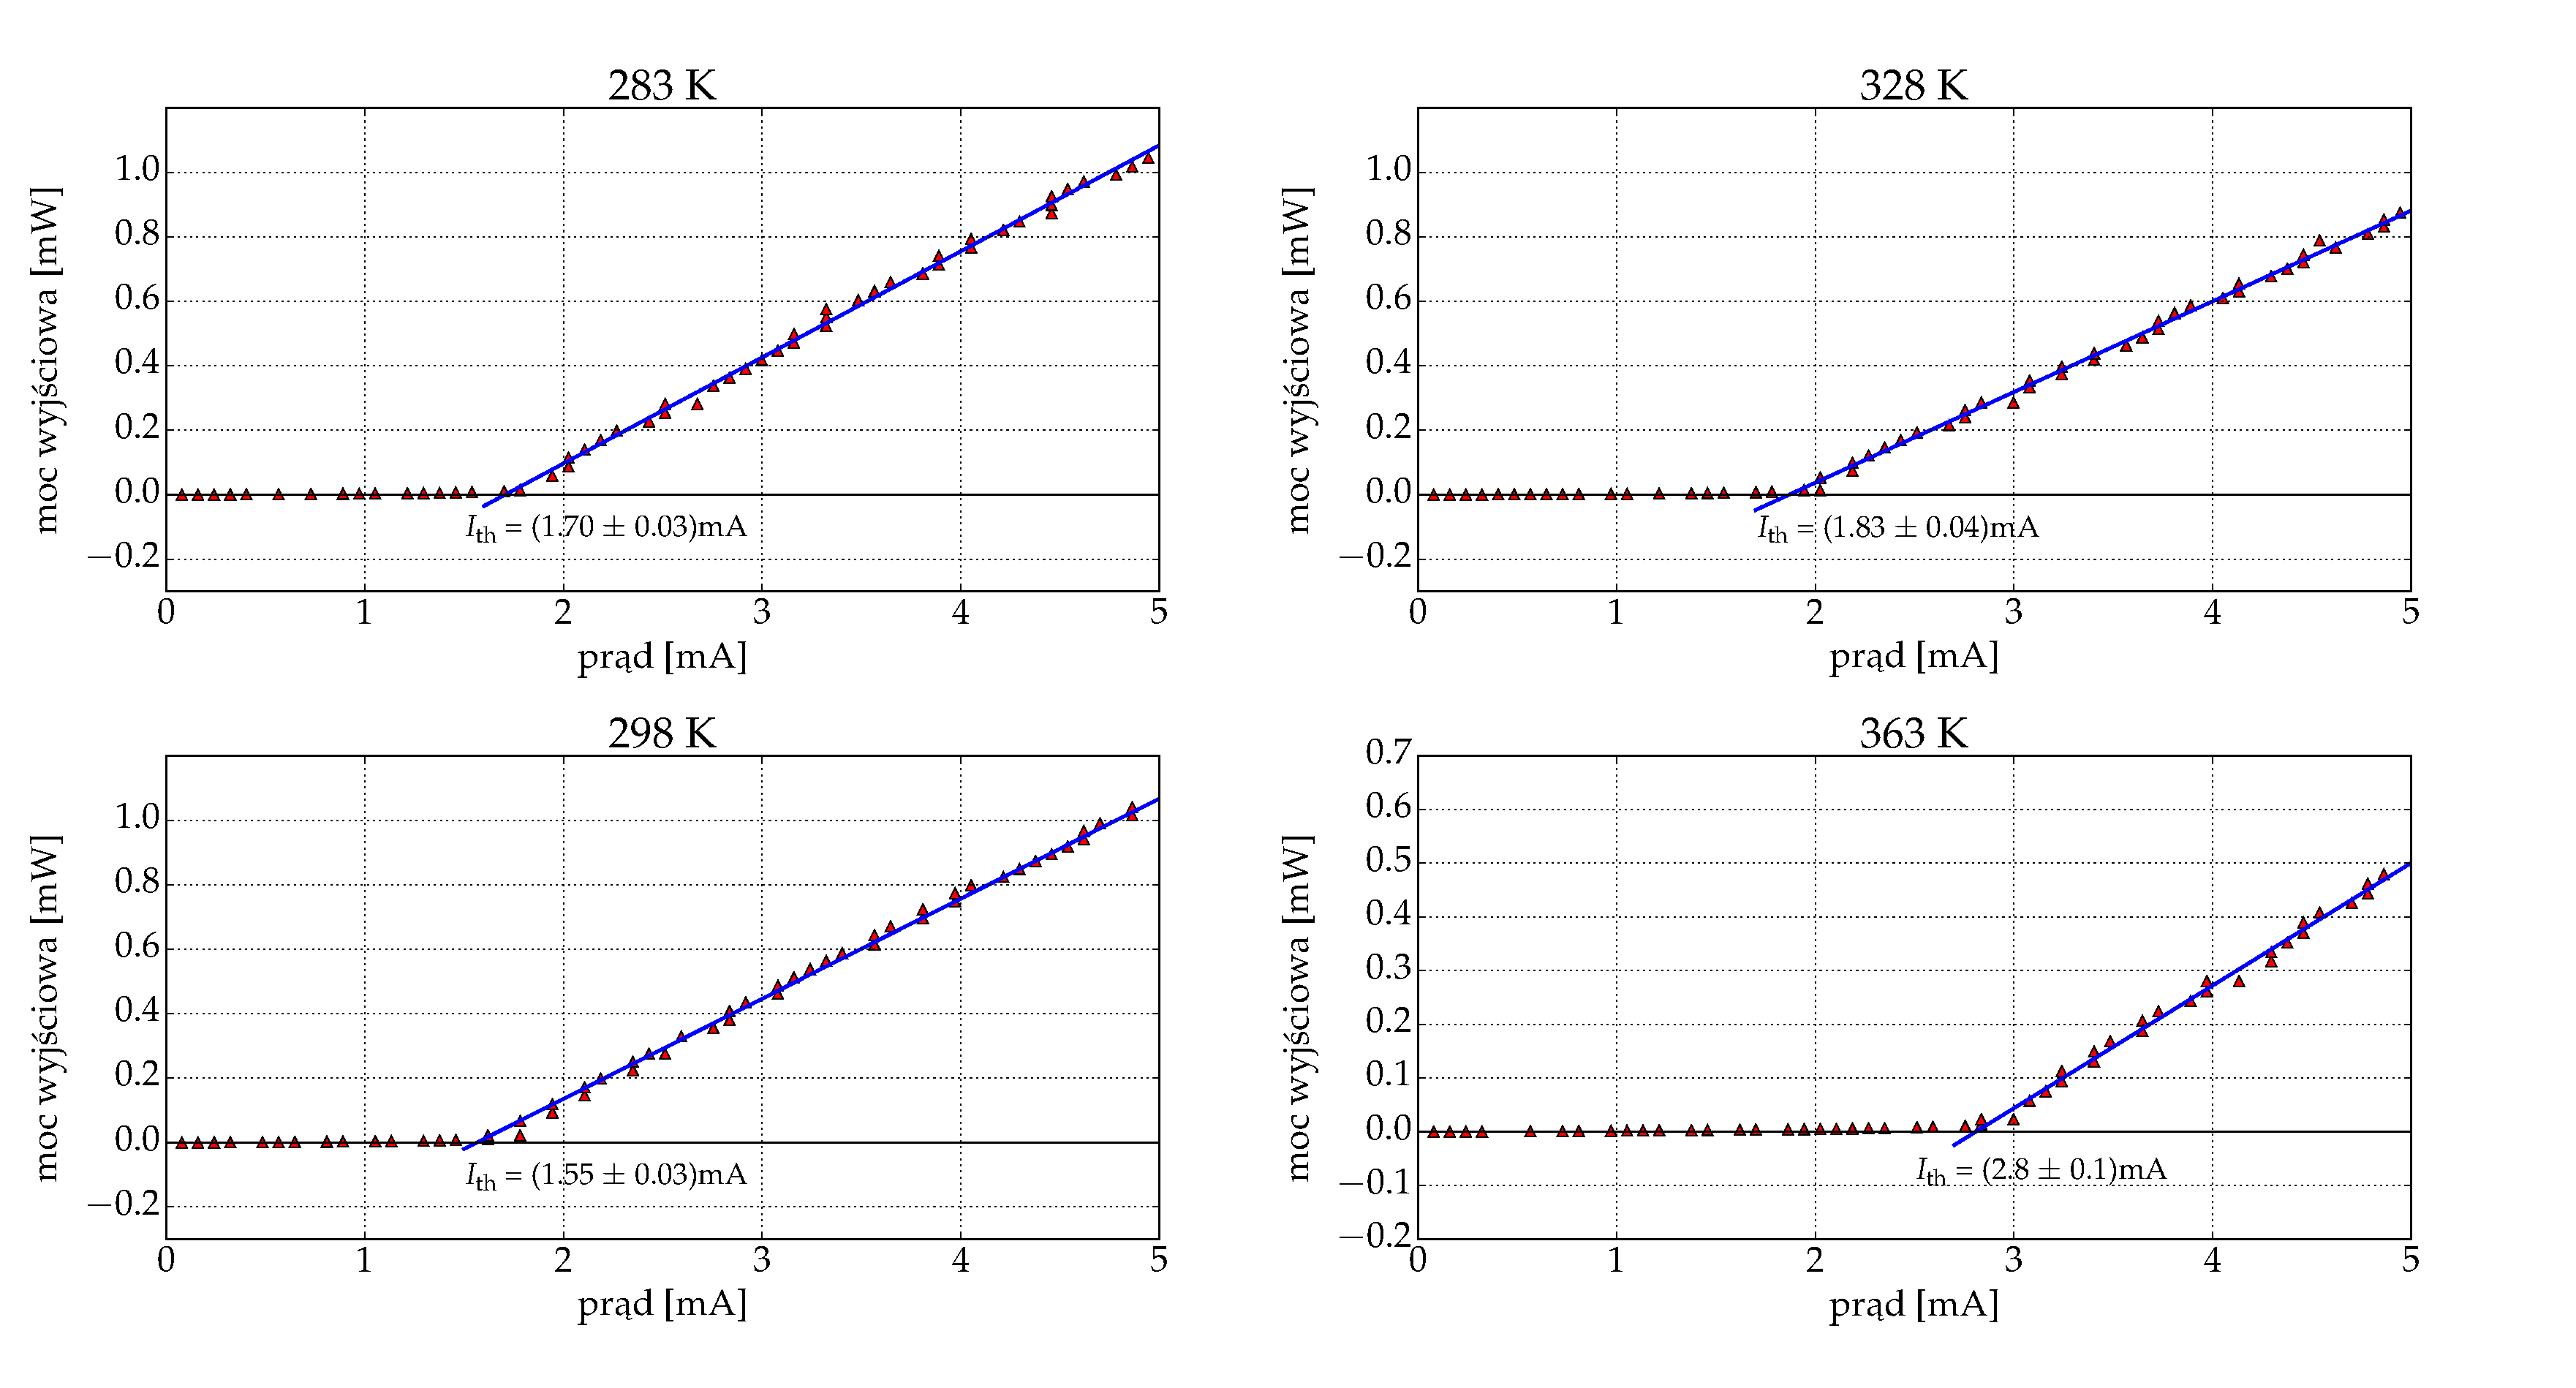
\includegraphics[scale=0.30]{plot_vcsel_850/plot_fit_i_th.eps}
  \caption{Wykres prądu progowego od temperatury z wyznaczonymi progami prądu dla lasera VCSEL 850\,nm.}
  \label{vcsel_850_rys_6}
\end{figure}
\begin{figure}
\center
  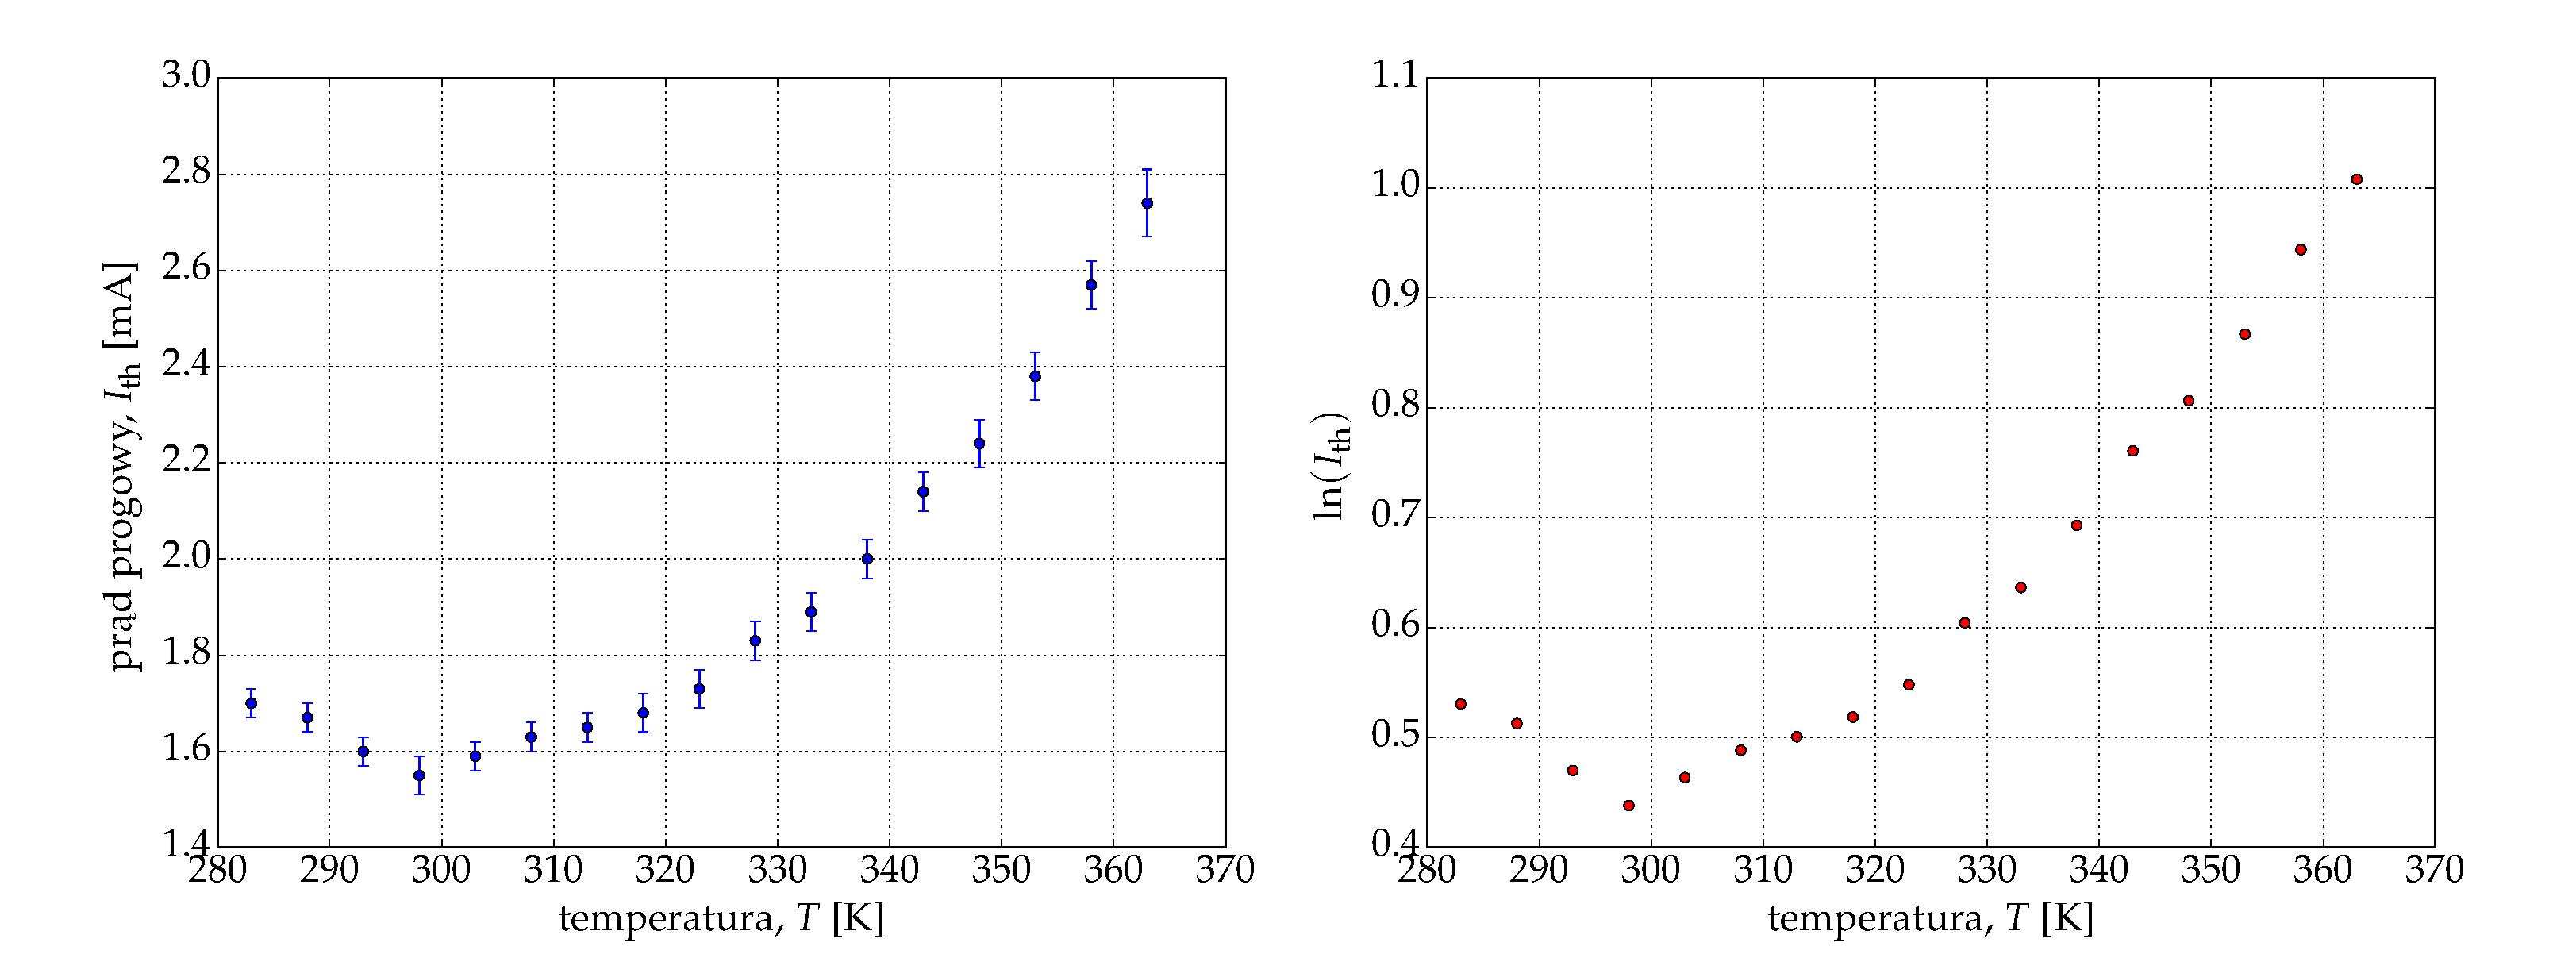
\includegraphics[scale=0.30]{plot_vcsel_850/plot_temp_i_th_log_lin.eps}
  \caption{Wykres prądu progowego od temperatury dla lasera VCSEL 850\,nm.}
  \label{vcsel_850_rys_7}
\end{figure}
%\begin{figure}
%\center
%  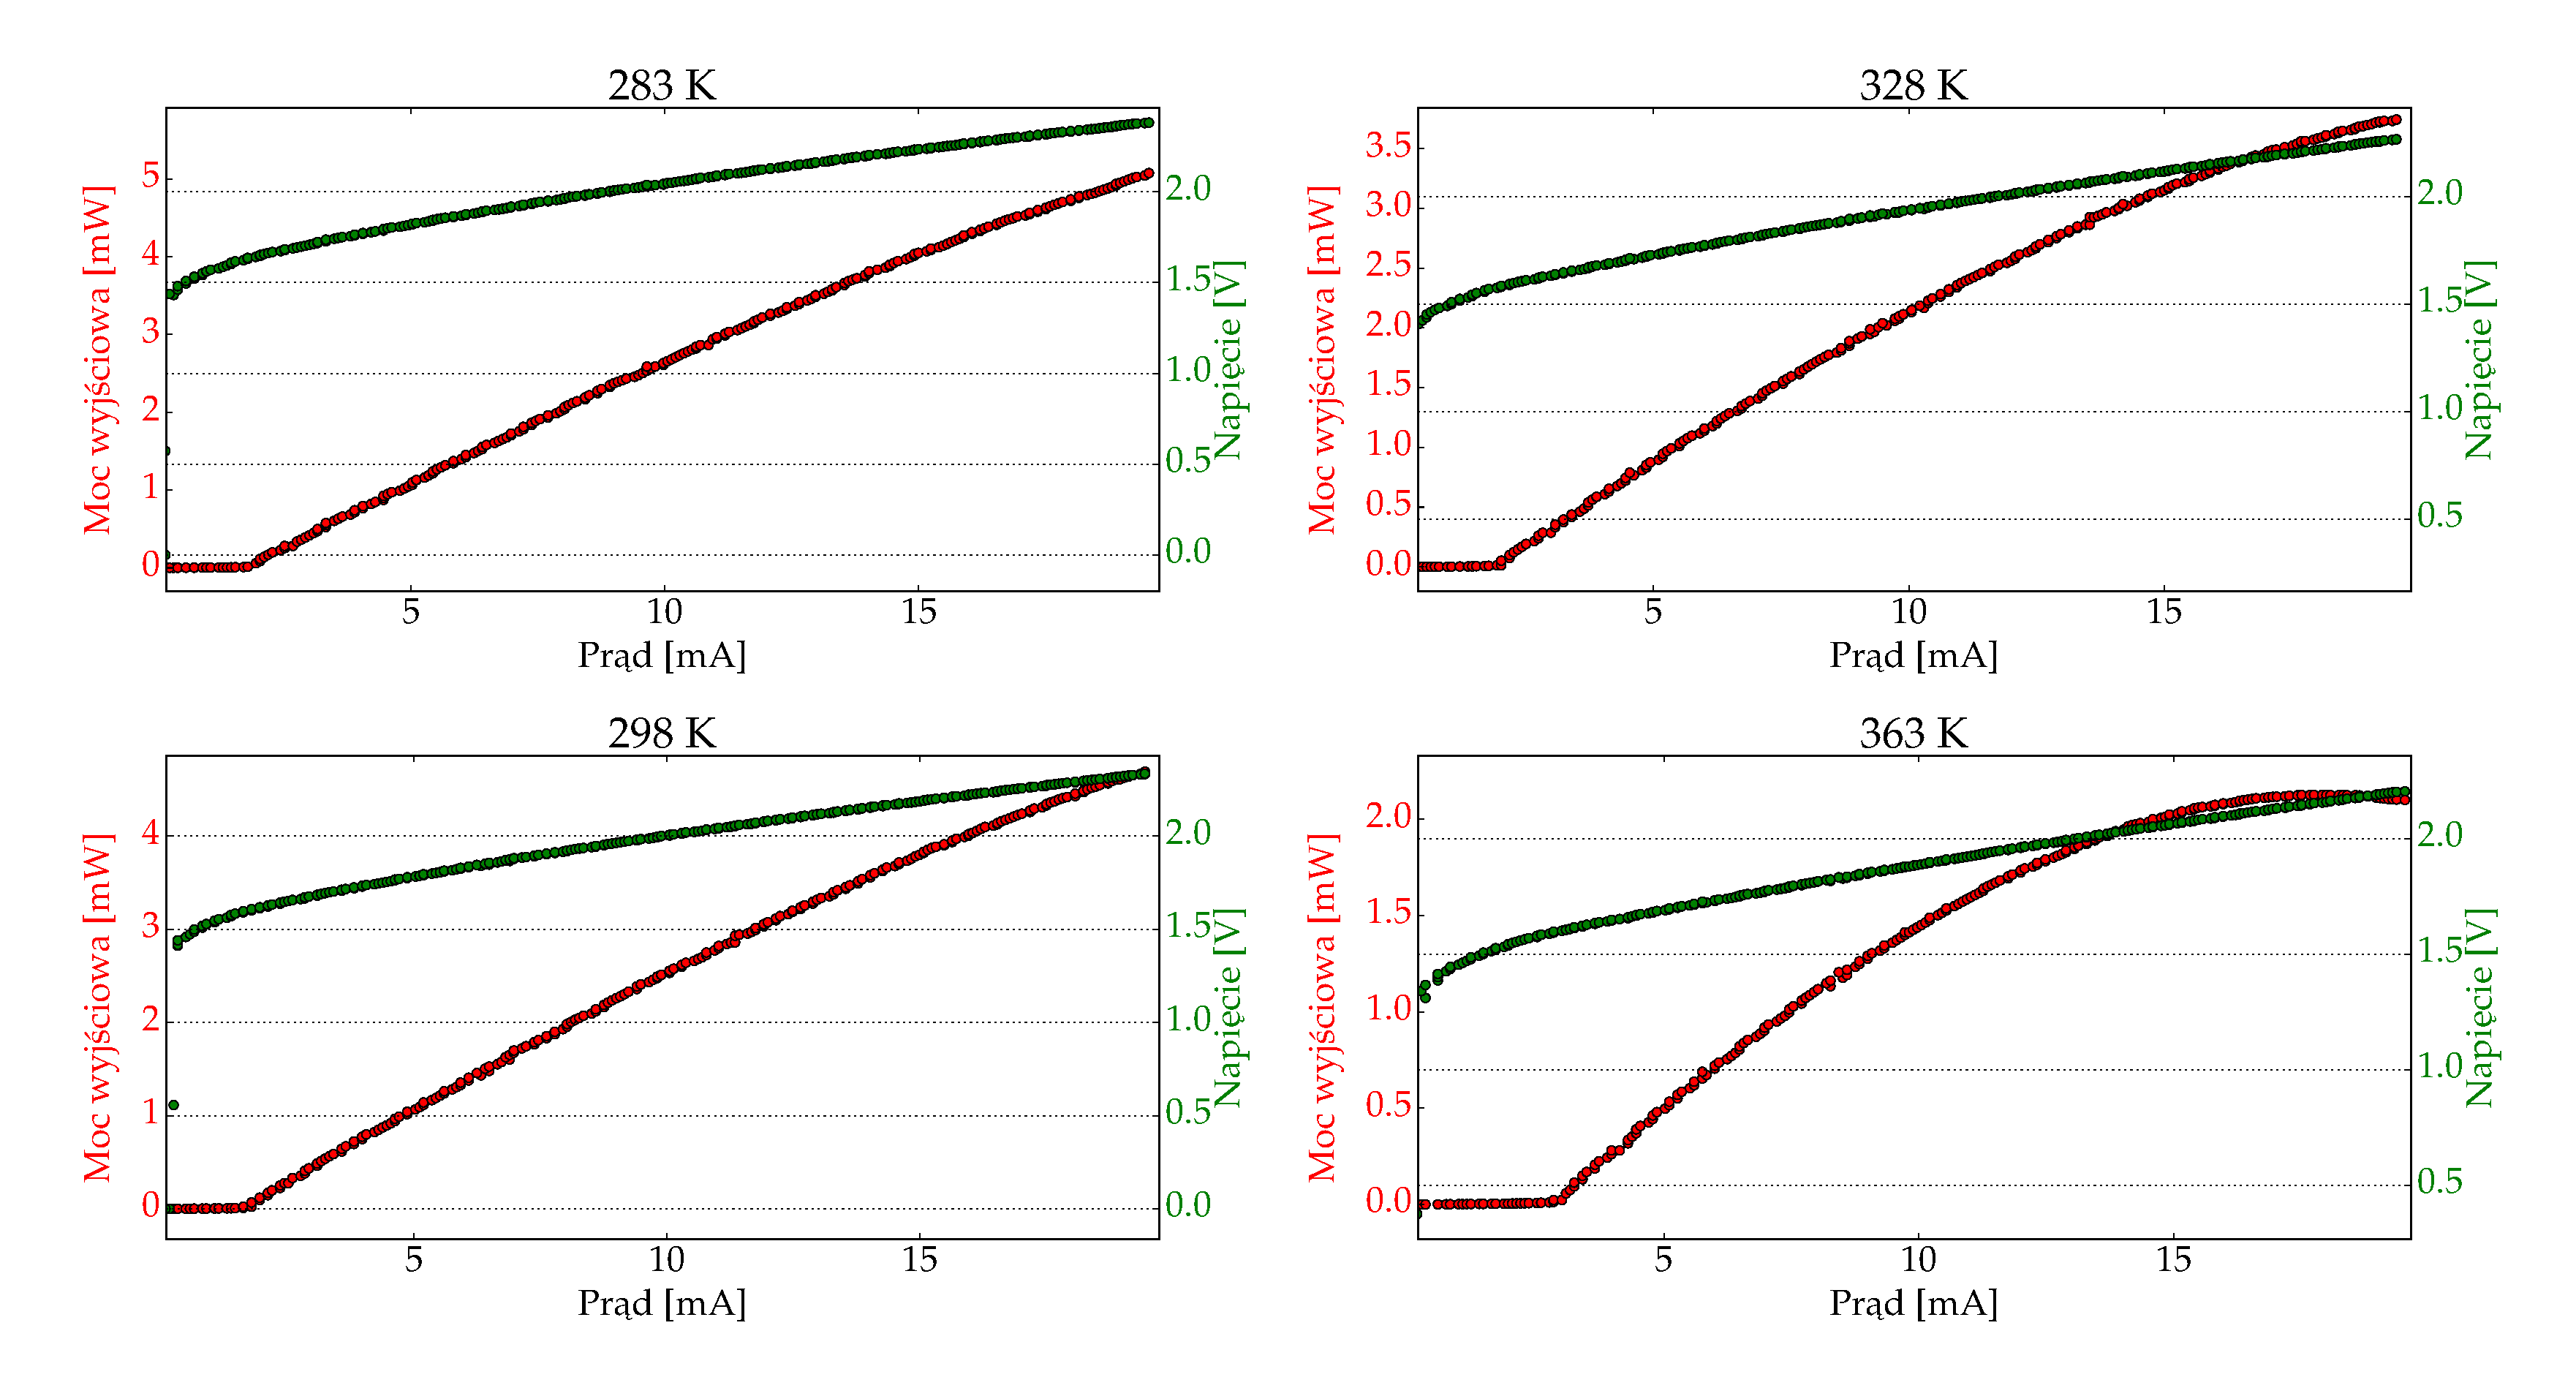
\includegraphics[scale=0.30]{plot_vcsel_850/plot_ivl_4.eps}
%  \caption{Sprawność VCSEL 850.}
%  \label{vcsel_850_rys_1}
%\end{figure}
\begin{figure}
\center
  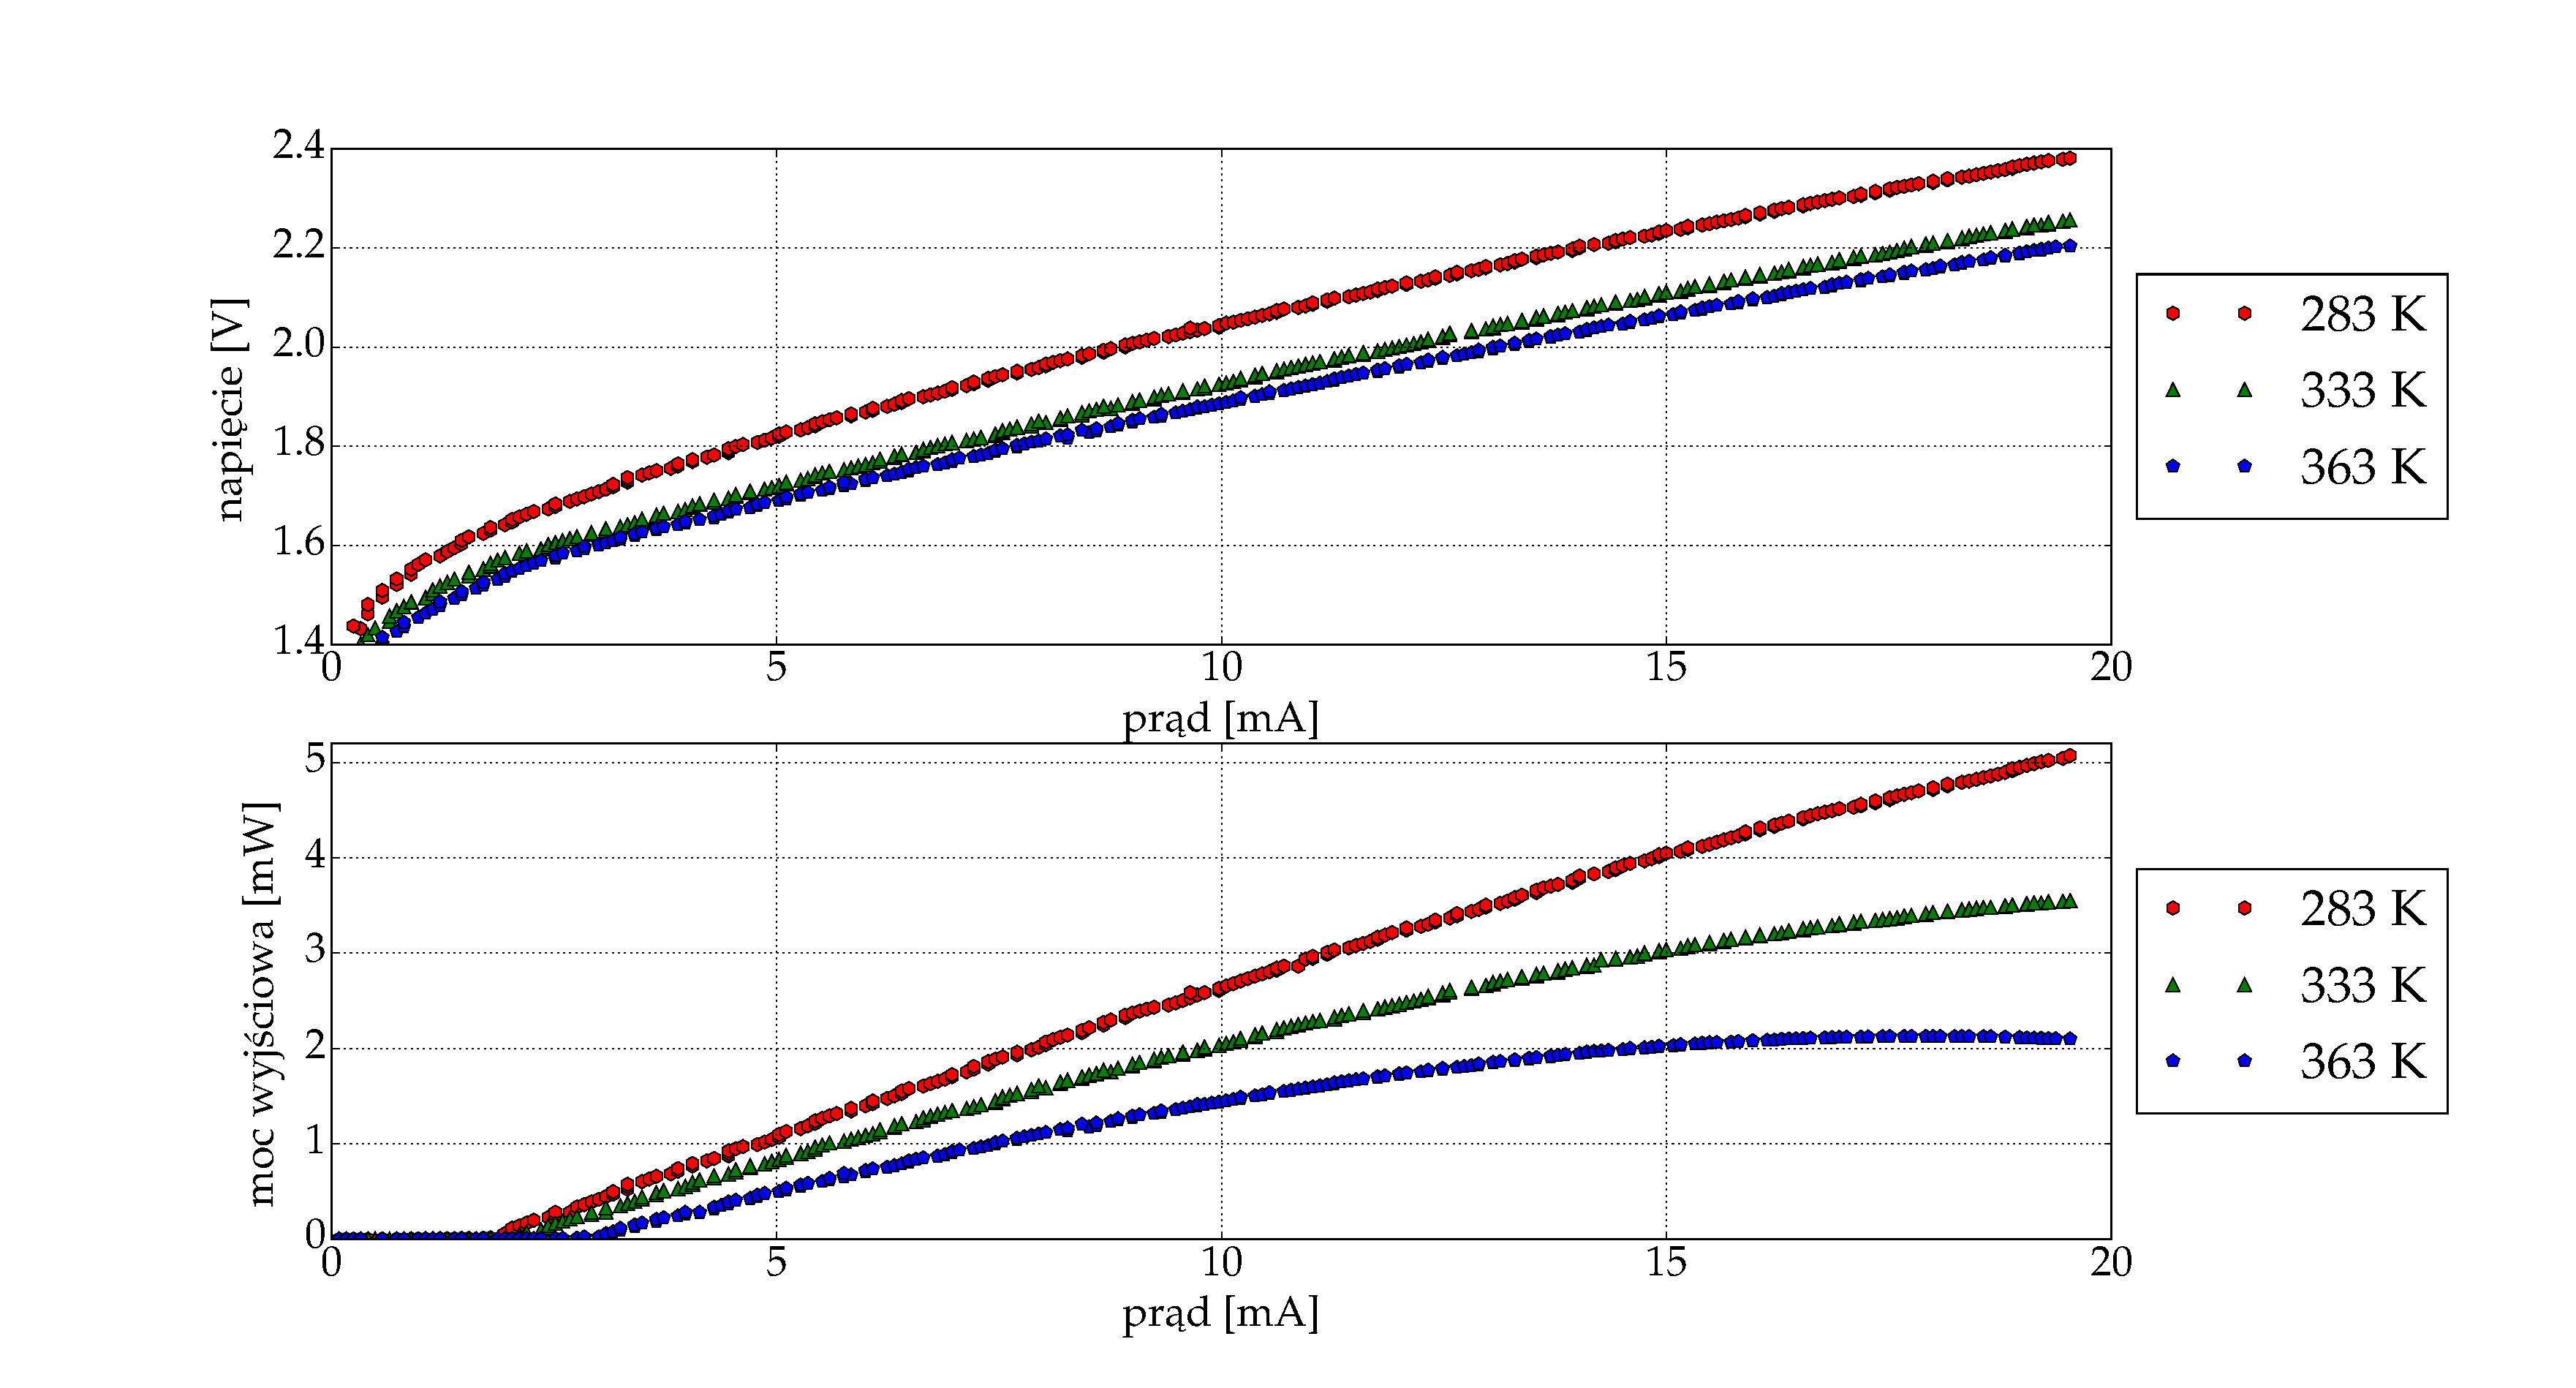
\includegraphics[scale=0.30]{plot_vcsel_850/plot_power_voltage.eps}
  \caption{Wykres napięcia na laserze i mocy wyjściowej w funkcji prądu od temperatury chłodnicy dla lasera VCSEL 850\,nm.}
  \label{vcsel_850_rys_2}
\end{figure}
%\begin{figure}
%\center
%  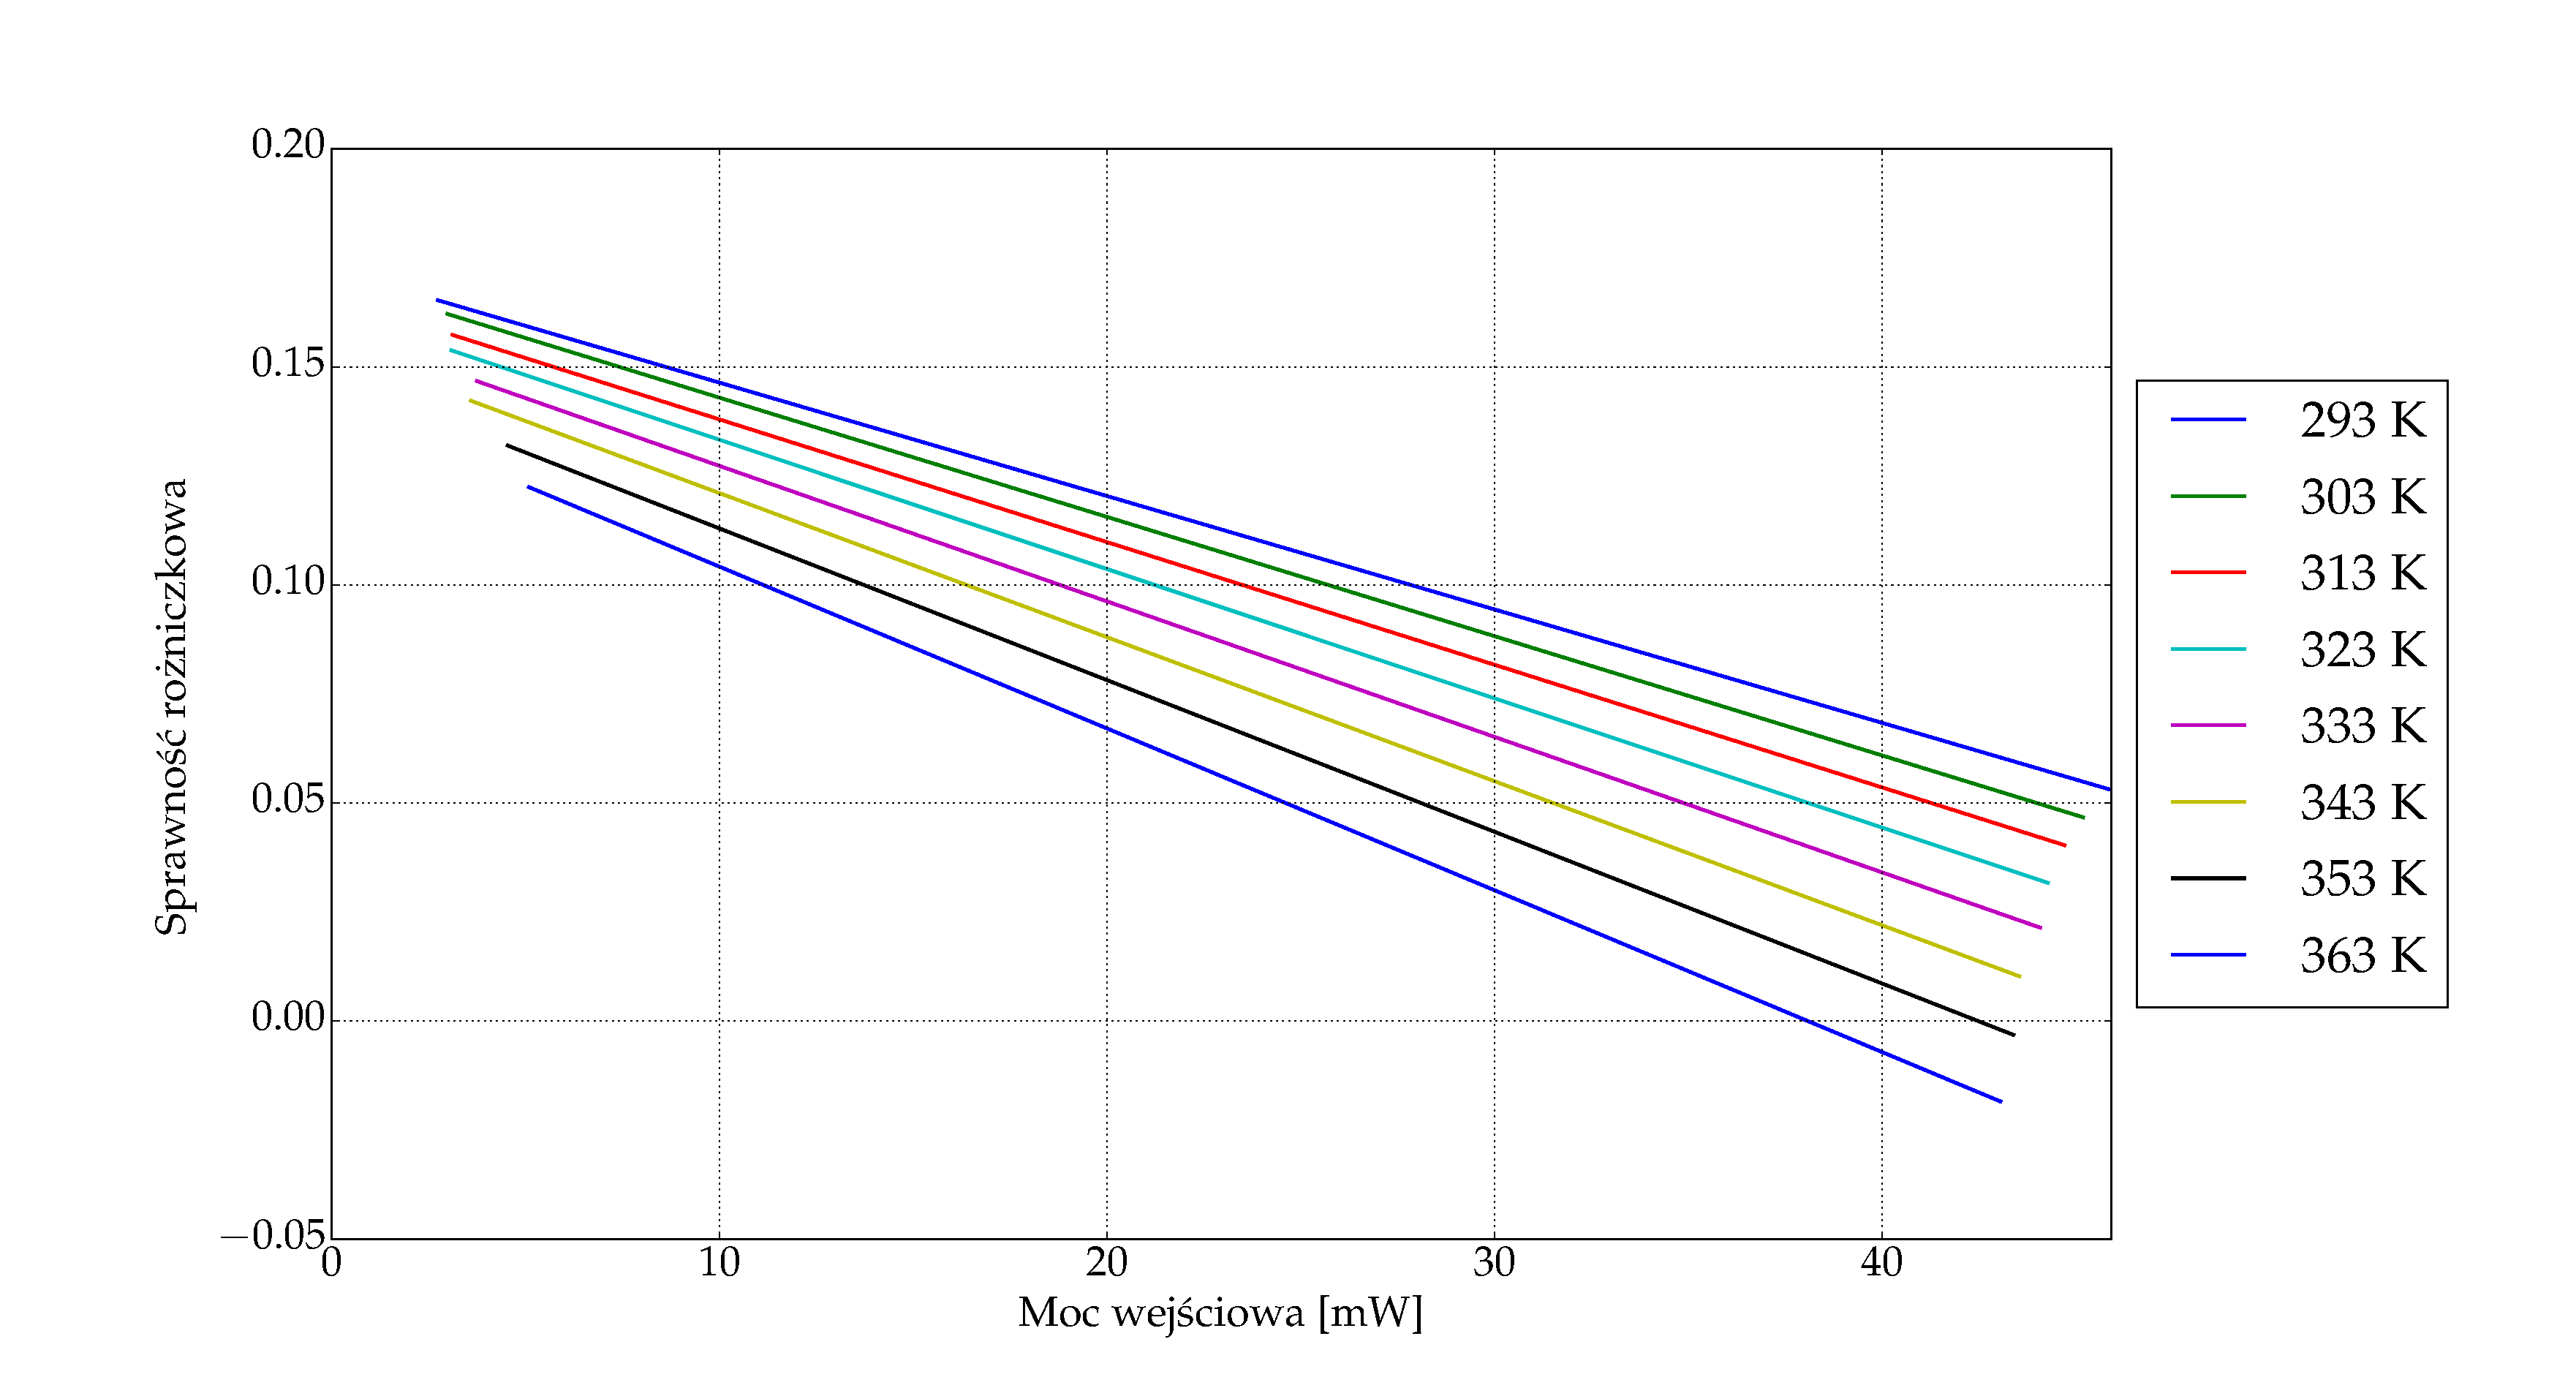
\includegraphics[scale=0.30]{plot_vcsel_850/plot_eff_all_via_power.eps}
%  \caption{Sprawność VCSEL 850 w funkcji mocy wejściowej.}
%  \label{vcsel_850_rys_4}
%\end{figure}
%\begin{figure}
%\center
%  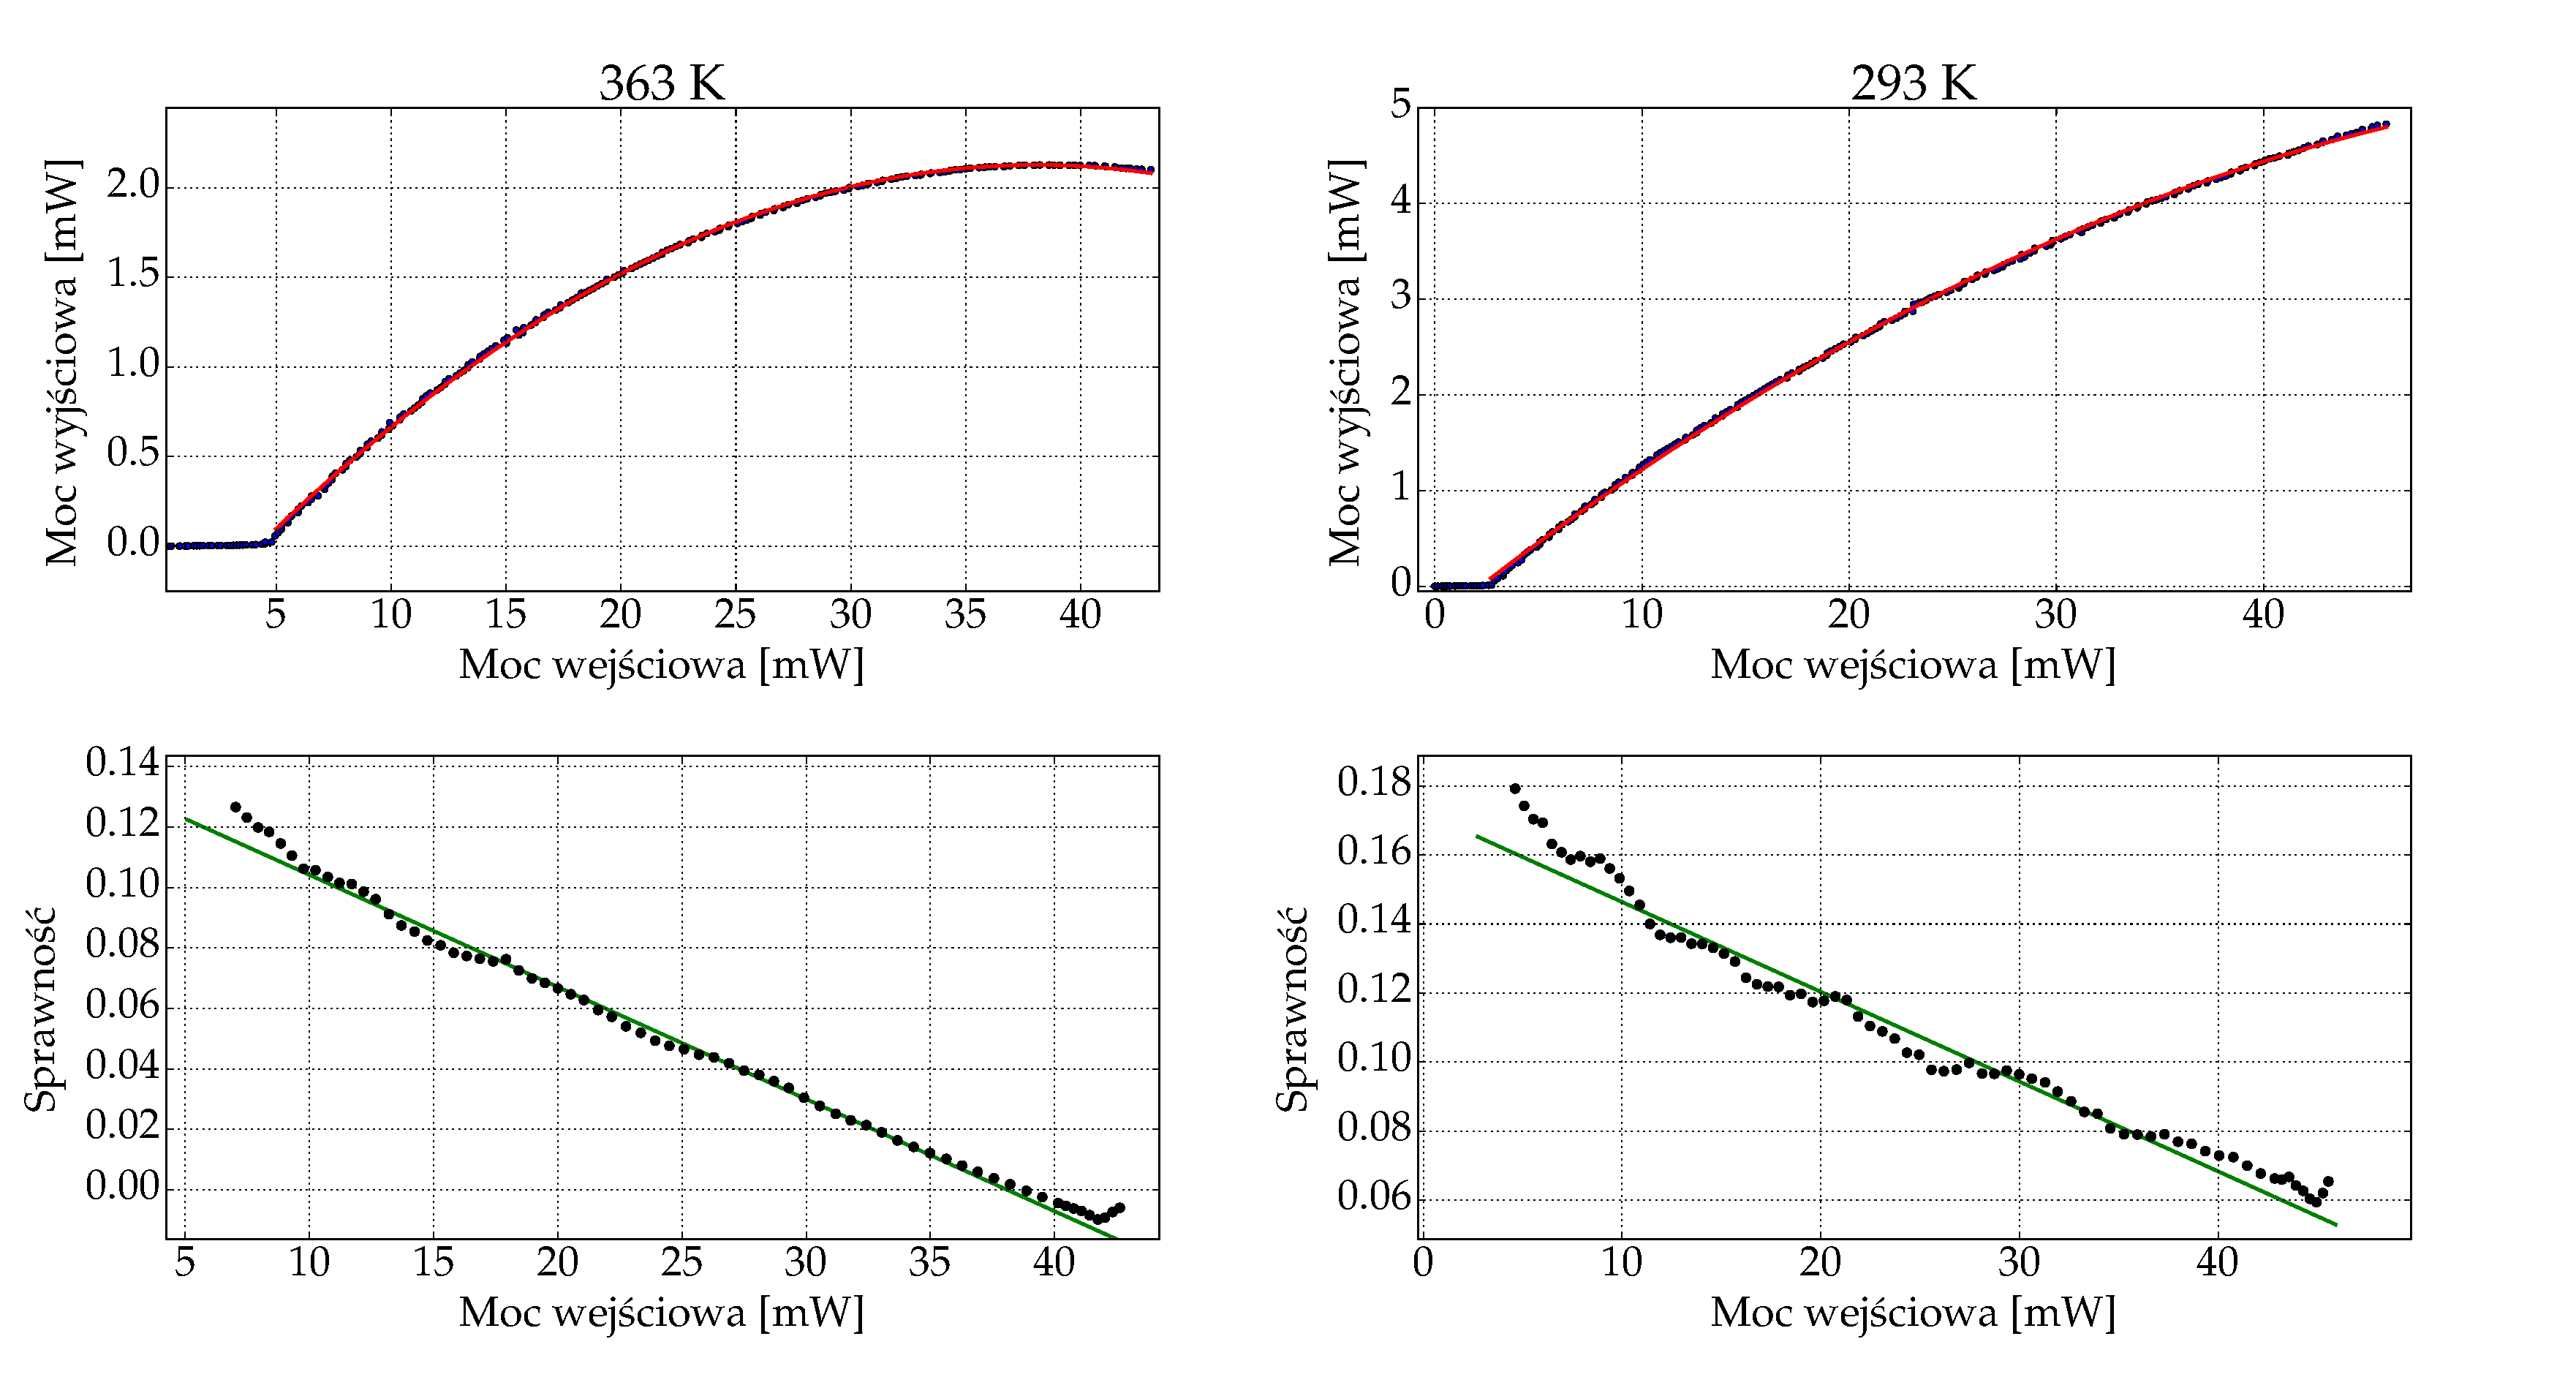
\includegraphics[scale=0.30]{plot_vcsel_850/plot_eff_20_90_via_power.eps}
%  \caption{Sprawność VCSEL 850 dla temperatury 293\,K i 363\,K.}
%  \label{vcsel_850_rys_5}
%\end{figure}
\begin{figure}
\center
  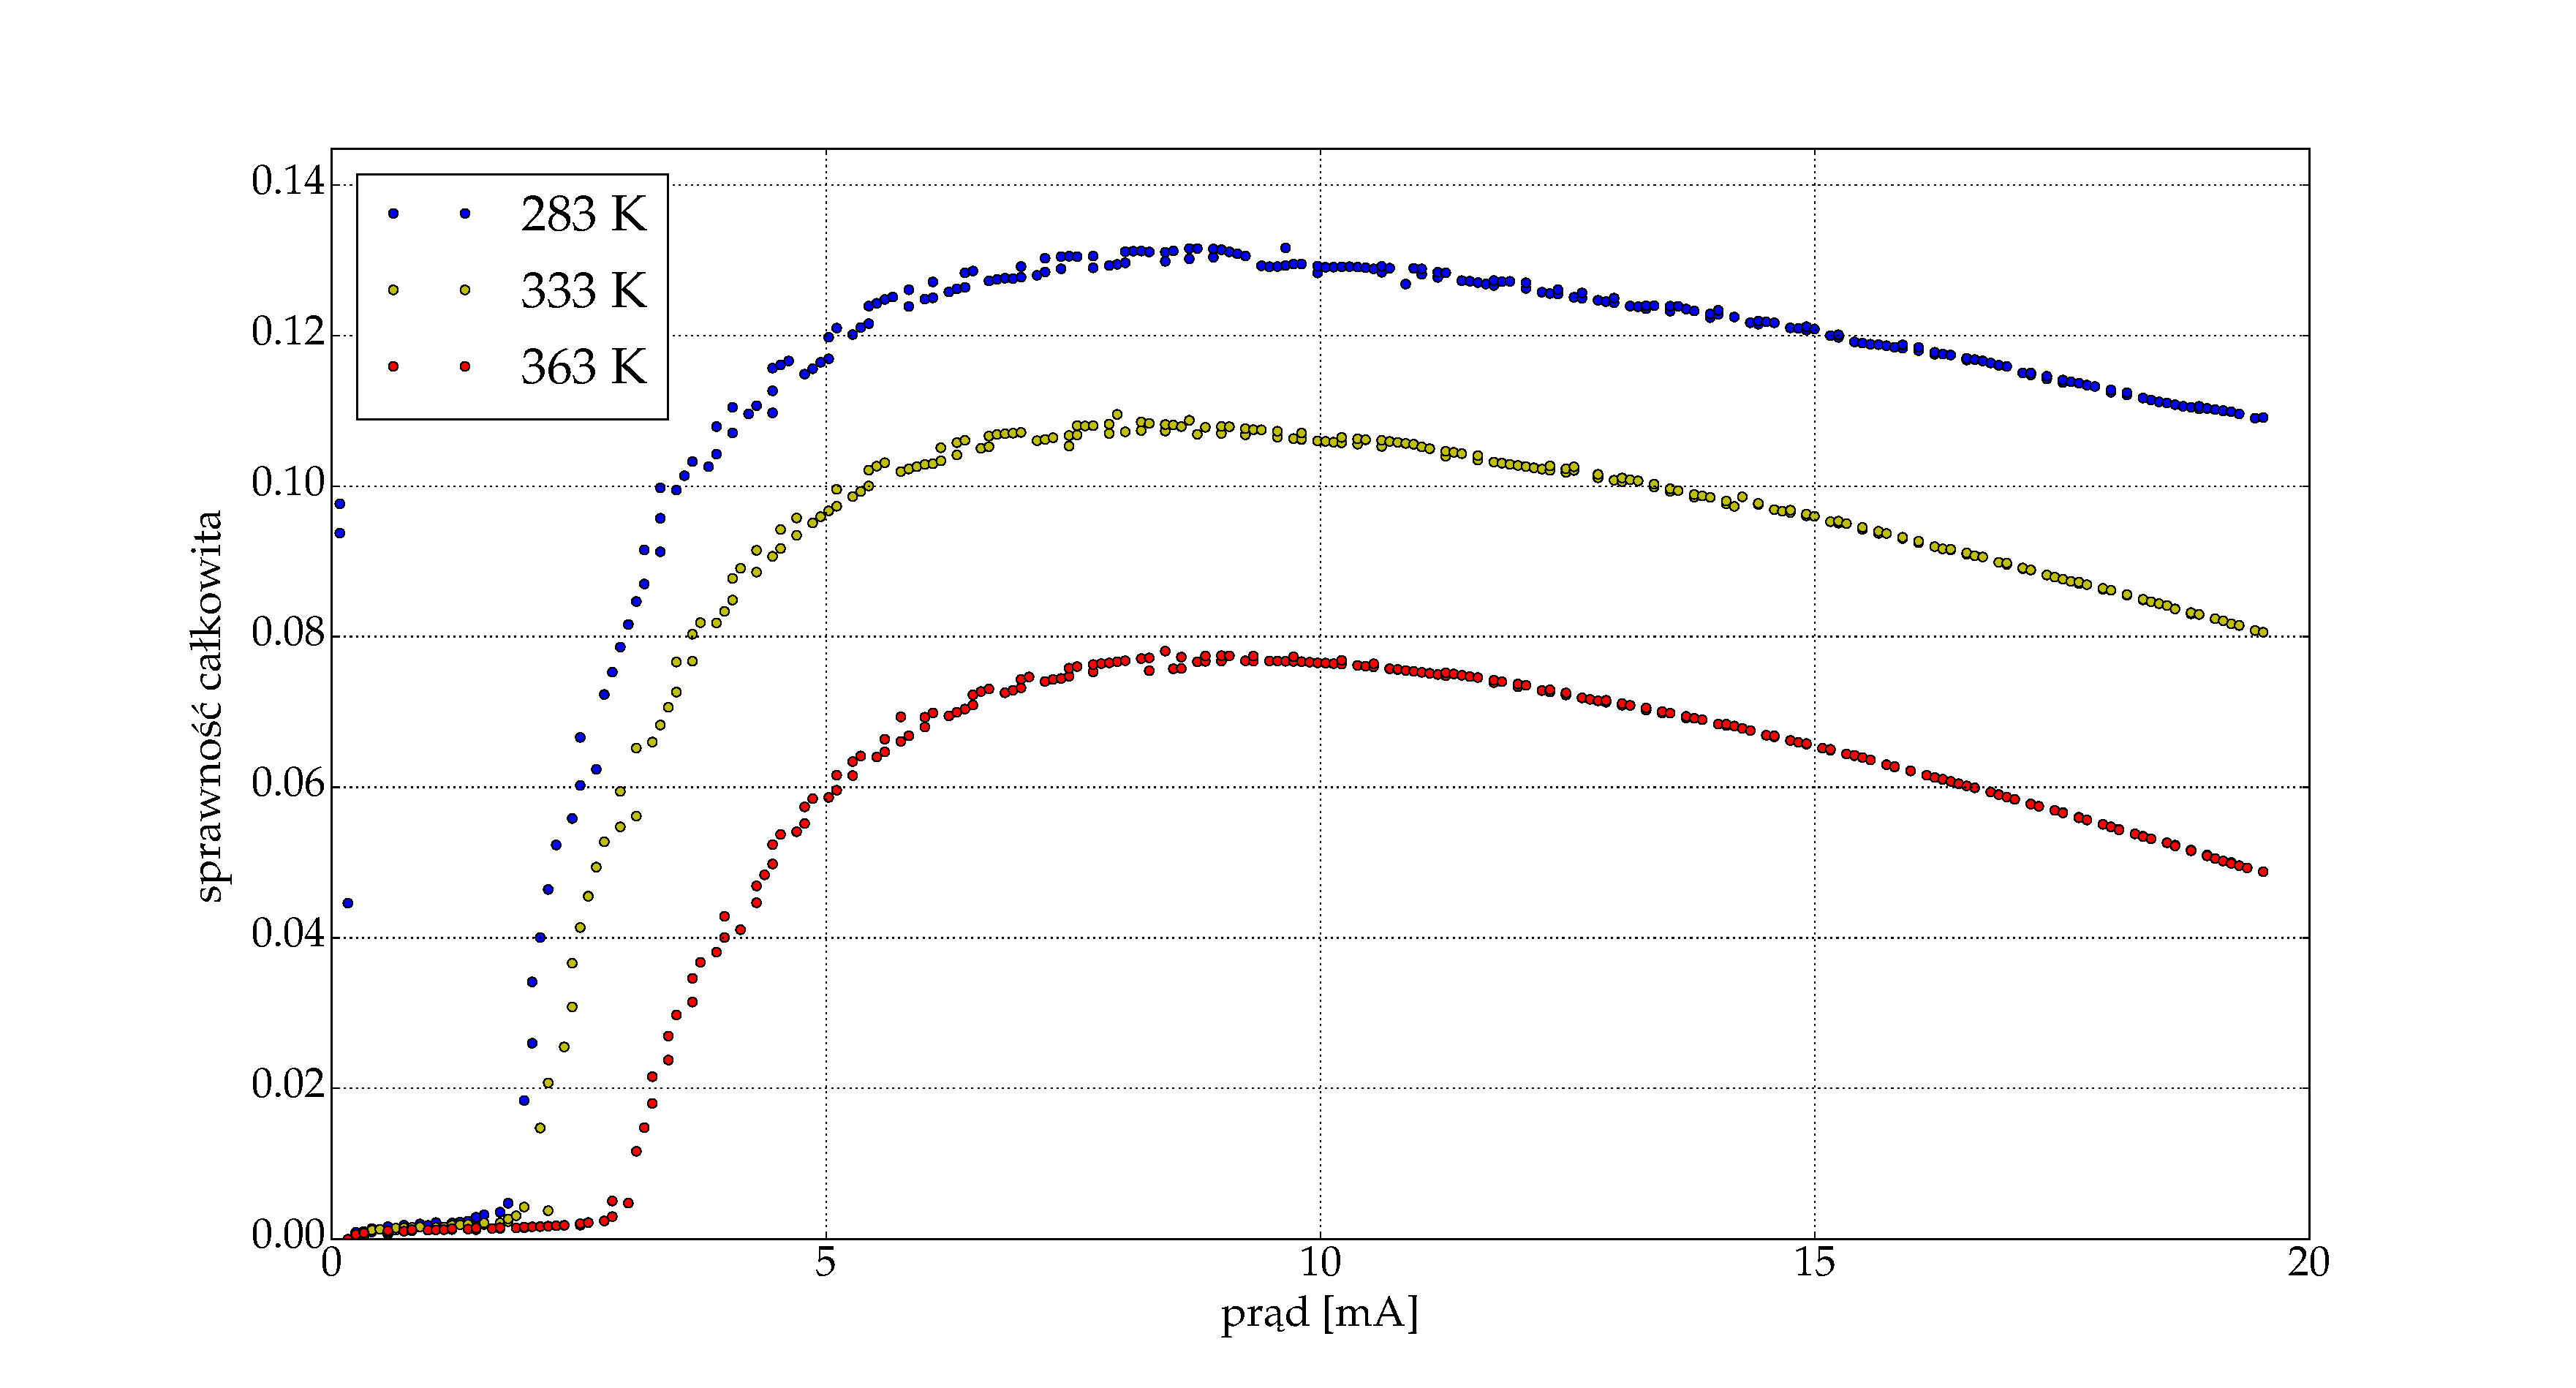
\includegraphics[scale=0.30]{plot_vcsel_850/plot_eff_wall.eps}
  \caption{Sprawność całkowita dla lasera VCSEL 850\,nm w różnych temperaturach.}
  \label{vcsel_850_rys_8}
\end{figure}
\begin{figure}
\center
  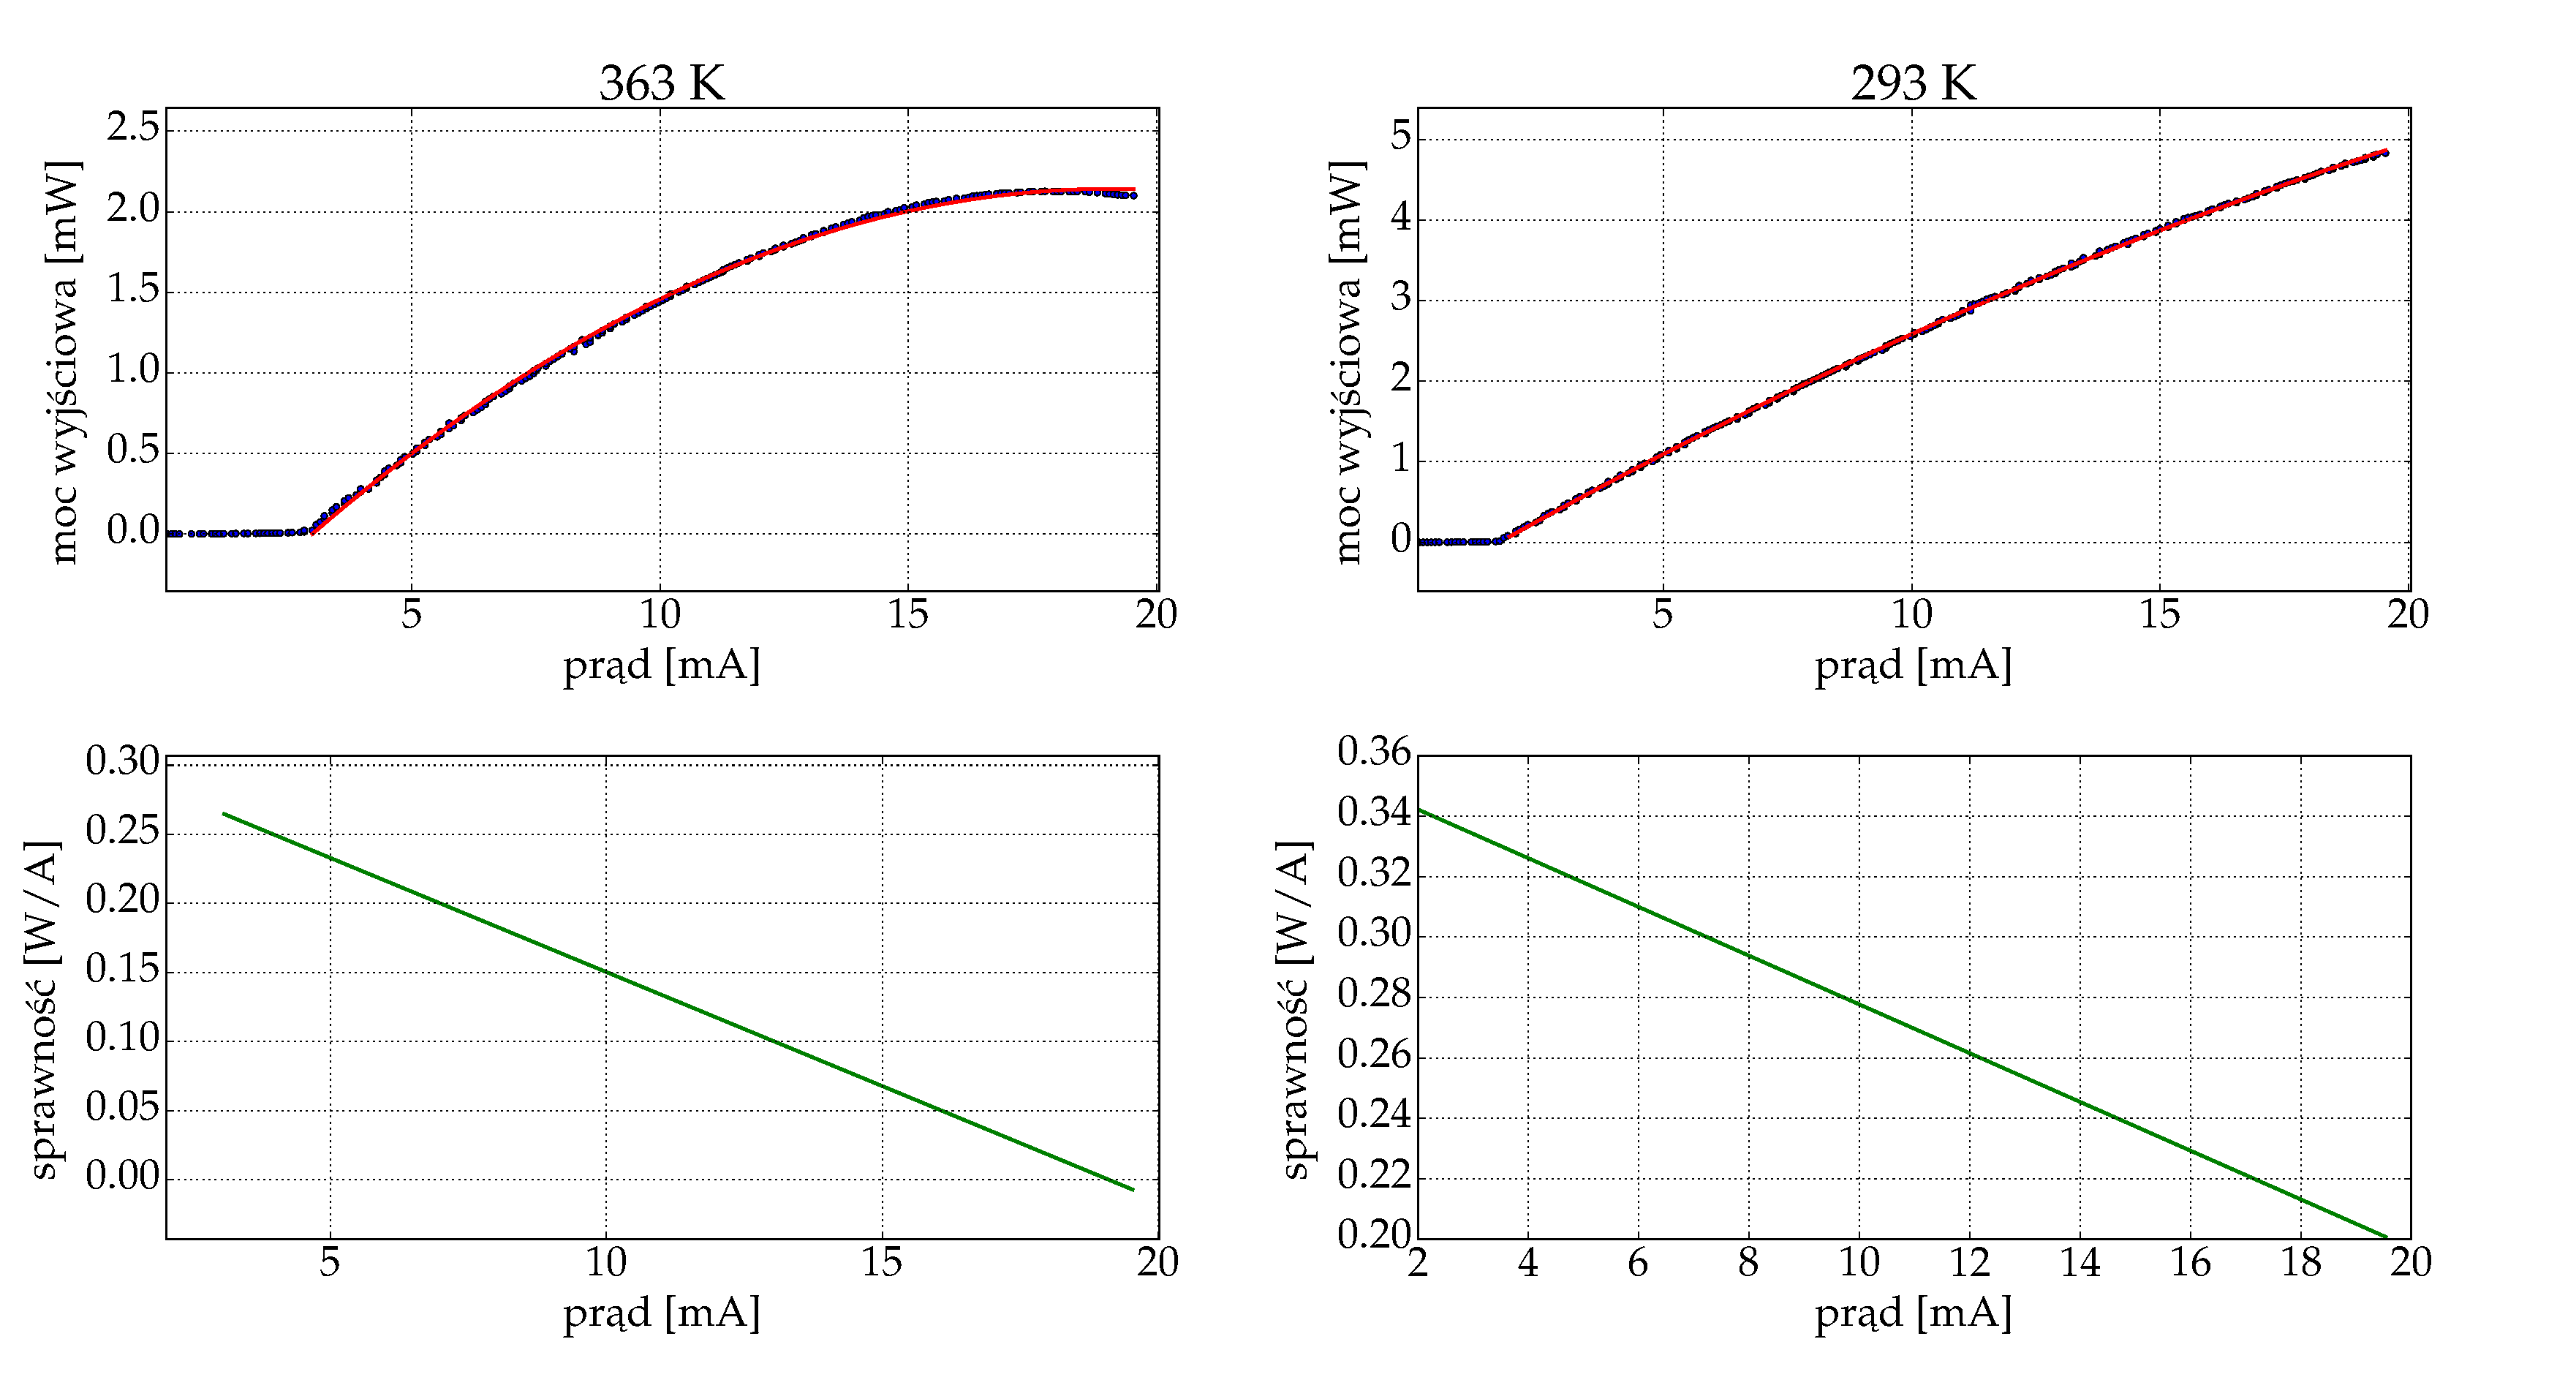
\includegraphics[scale=0.30]{plot_vcsel_850/plot_eff_all_via_current2.eps}
  \caption{Sprawność różniczkowa dla lasera VCSEL 850\,nm w różnych temperaturach.}
  \label{vcsel_850_rys_9}
\end{figure}
\begin{figure}
\center
  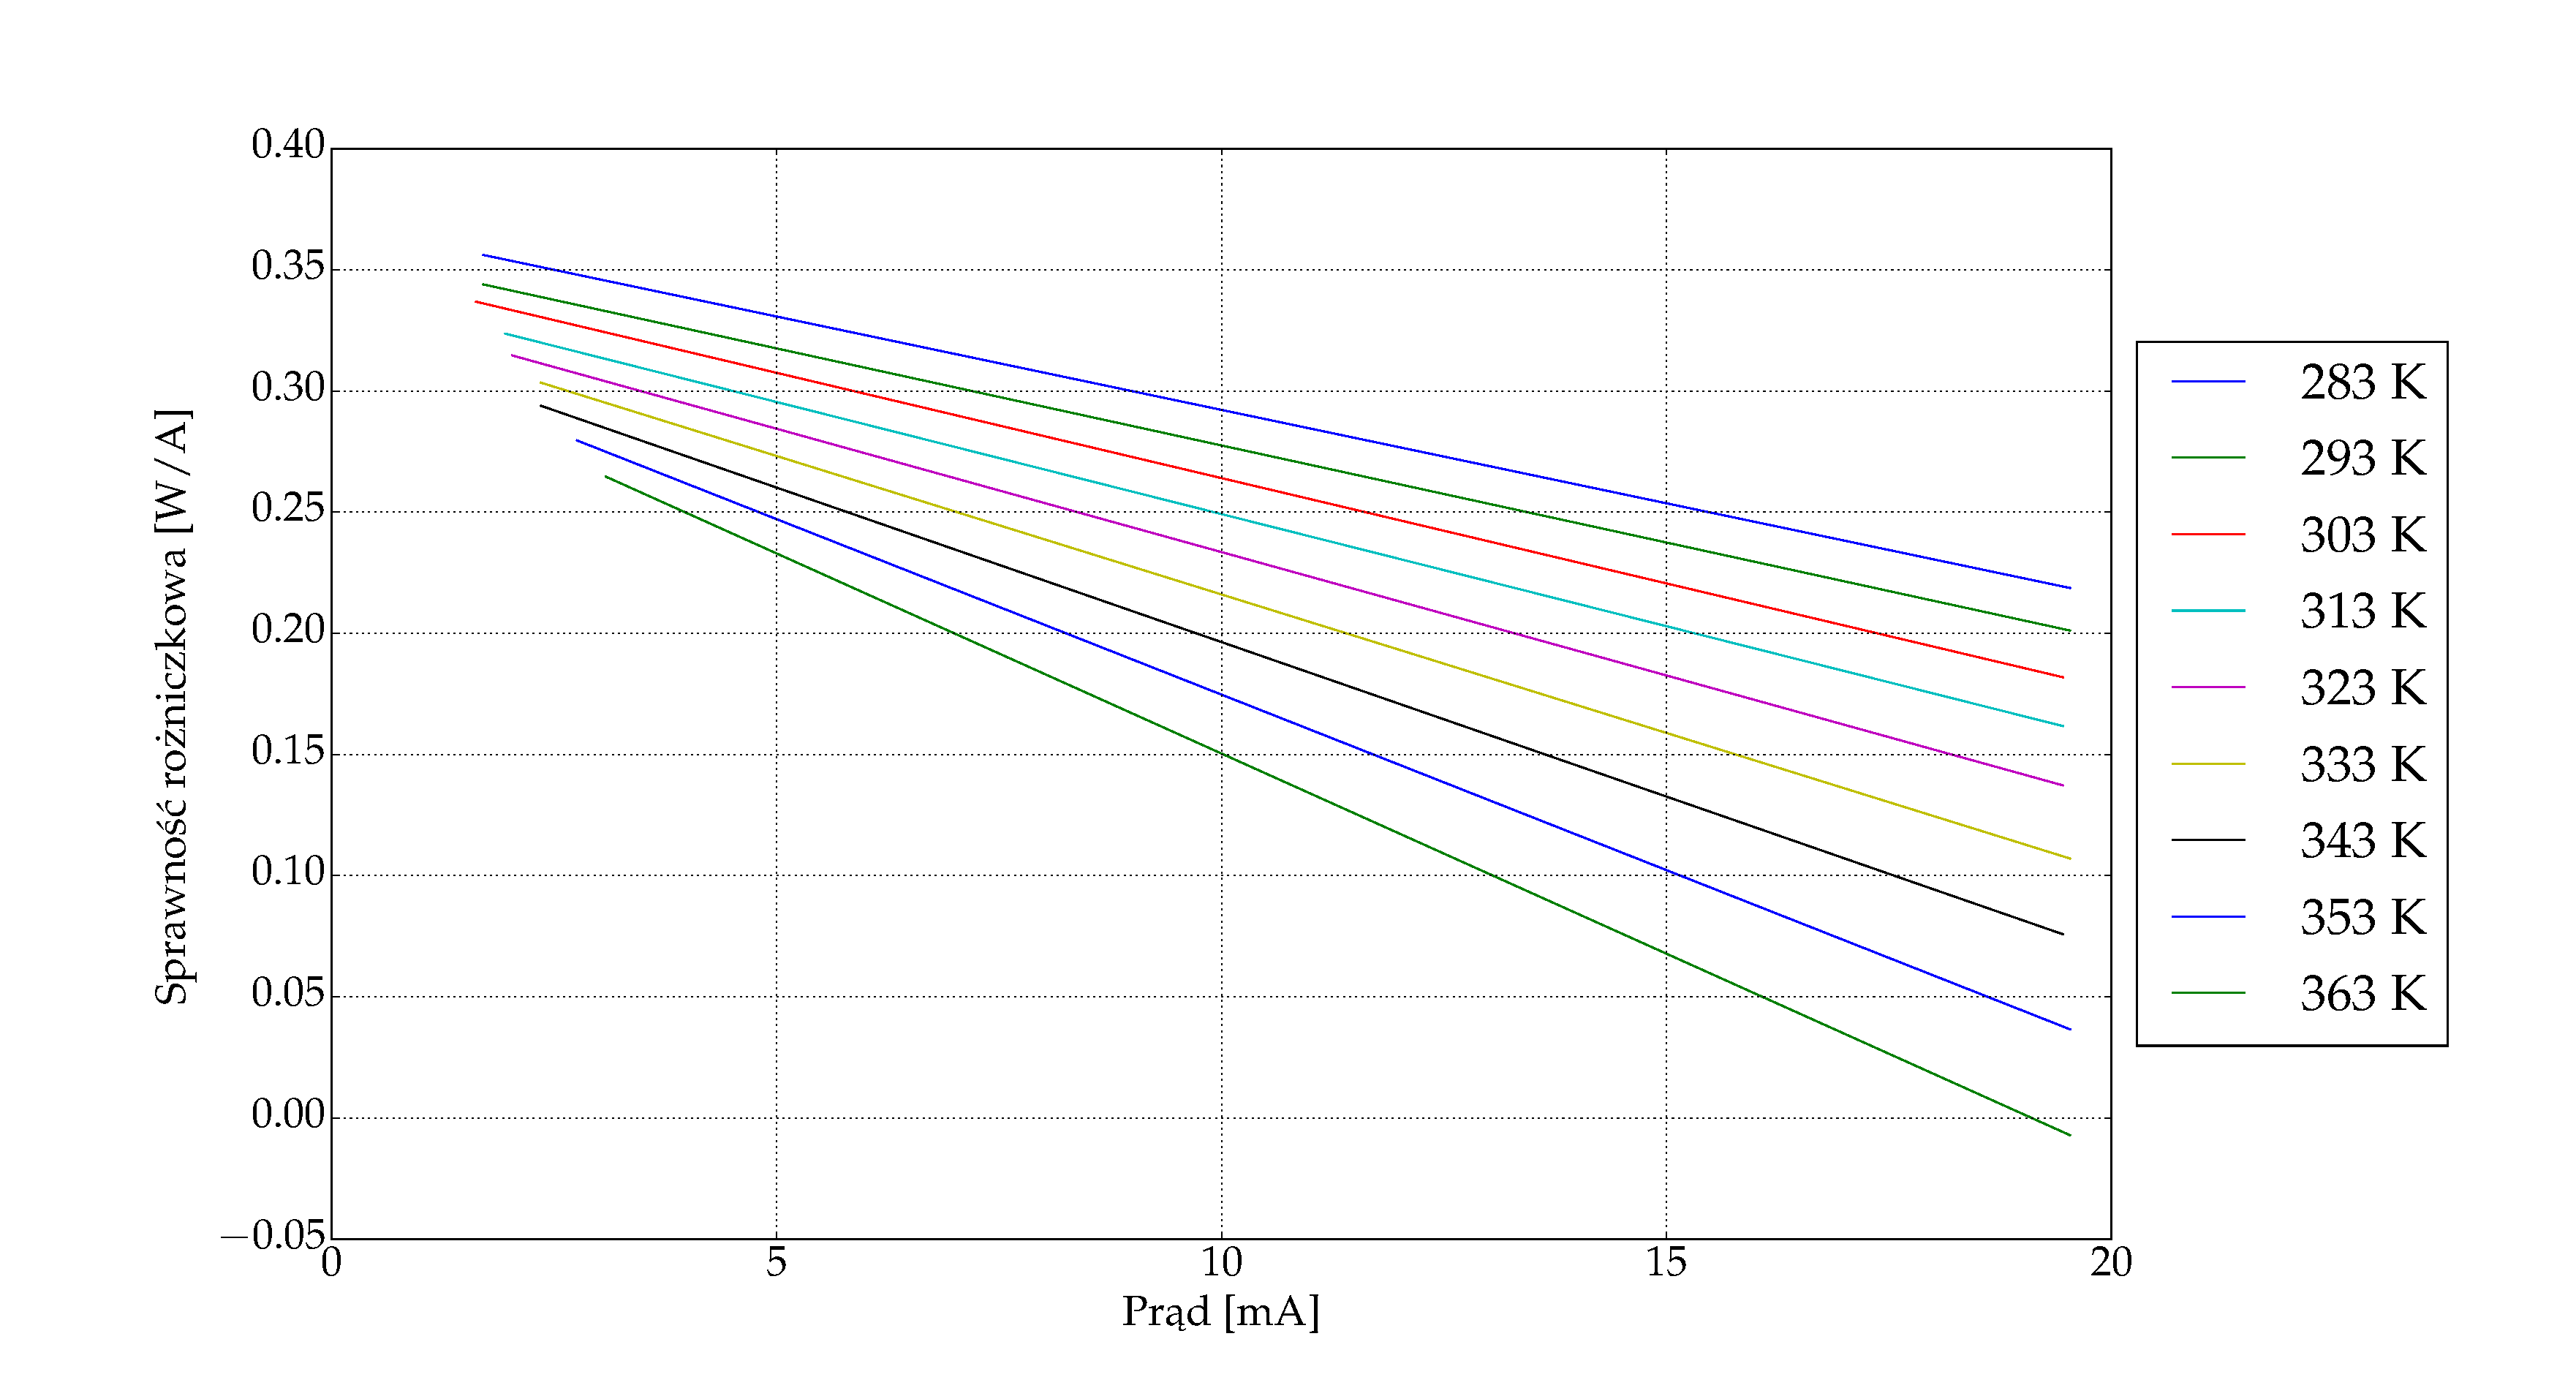
\includegraphics[scale=0.30]{plot_vcsel_850/plot_eff_all_via_current.eps}
  \caption{Sprawność VCSEL 850 w funkcji prądu.}
  \label{vcsel_850_rys_3}
\end{figure}
\newpage
\section{Omówienie wyników}
Dzięki analizie sporządzonych wykresów można dojść do następujących konkluzji:
\begin{itemize}
\item Analizując wykres napięcia na laserze od prądu wejściowego przedstawiony na rysunku~\ref{vcsel_850_rys_1} oraz~\ref{vcsel_850_rys_2} można zauważyć, że wraz ze wzrostem temperatury na chłodnicy
maleje opór lasera. Także, wraz z wyższą temperaturą chłodnicy maleje moc wyjściowa lasera.
\item Wykres na rysunku~\ref{vcsel_850_rys_3} przedstawia sprawność różniczkowa lasera w funkcji prądu wejściowego od temperatury na chłodnicy, jak wynika z wykresu im
wyższa temperatura tym sprawność lasera mniejsza.
\item Wykres na rysunku~\ref{vcsel_850_rys_4} przedstawia sprawność różniczkowa lasera w funkcji mocy wejściowej od temperatury na chłodnicy, jak wynika z wykresu im
wyższa temperatura tym sprawność lasera mniejsza.
\item Wykres na rysunku~\ref{vcsel_850_rys_5} przedstawia w górnej cześci zależności mocy wyjściowej od mocy wejściowej.
\item Wykres na rysunku~\ref{vcsel_850_rys_7} pokazuje zależności prądu progowego od temperatury. Jak widzimy przy temperaturach (280-300)\,K
wraz ze wzrostem temperatury maleje wartość prądu progowego, natomiast dla temperatur $>$ 300\,K im wyższa temperatura to zwiększa się
wartość prądu progowego.
\item Wykres na rysunku~\ref{vcsel_850_rys_8} przedstawia sprawnośc całkowitą lasera dla trzech temperatur: 283\,K, 333\,K, 363\,K. Analizując ten wykres
dochodzę do wniosku, że im wyższa temperatura tym sprawnośc mniejsza.
\item Wykres na rysunku~\ref{vcsel_850_rys_9} przedstawia sprawności różniczkowe dla dwóch temperatur. W górnej cześci przedstawiona jest charakterystyka
wyjściowa z dopasawaną funkcją w postaci wielomianu stopnia drugiego. Pochodna tej funkcji jest sprawnością rożniczkową. Na dolnym wykresie przedstawiona
jest sprawność w postaci prostej będącej pochodną dopasowanej funkcji. Natomiast czarne kropki przedstawiają sprawność powstałą w wyniku obliczenia pochylenia
10 punktów przefiltrowanych co 3 punkty.
\end{itemize}
